\chapter{\iflanguage{ngerman}{Herausforderungen}{Challenges}}
\label{sec:overview}

Der Hybride OP-Saal bringt Vorteile für zukünftige Entwicklung des Operationssaals. Dennoch kommen bei der Planung, Umsetzung und Vernetzung einige Herausforderungen auf, die berücksichtigt werden müssen. 
Nicht alle Aspekte sind positiv und ob sich ein Hybrider OP-Saal tatsächlich lohnt, muss validiert werden.

\subsection{Nachteile}

Der Hybride OP-Saal wird in erster Linie durch die bildgebenden Verfahren definiert. Wie bereits aus der Radiologie bekannt, müssen immer auch mögliche \glqq Mess-, Rekonstruktions- und Modellierungsfehler berücksichtigt werden\grqq{} \cite{DerDigitaleOperationssaal}. 
So können Partialvolumenartefakte (siehe Abb. \ref{fig:partial}) Grund dafür sein, dass Tumore in der falschen Größe dargestellt werden. Auch kann es vorkommen, dass kleine Läsionen (< 1cm) nicht immer in den CT-Bildern abgebildet werden. Diese möglichen Fehler müssen in der bereits komplexen und zeitaufwendigen Operationsplanung und späteren Durchführung berücksichtigt werden \cite{DerDigitaleOperationssaal}.

Hinzu kommt, dass Operationen im Hybriden OP-Saal teilweise unter laufender Röntgenkontrolle statt finden. Diese Strahlenbelastung betrifft nicht nur den Patienten sondern das gesamte behandelnde Team wird der durch den Patienten verursachten Streustrahlung ausgesetzt. Je nach Abstand, Winkel und Höhe zum Patienten während der Bildkontrolle, wird eine anwesende Person 9 bis 39\% der Strahlung ausgesetzt, die der Patient ausgesetzt wird (bei einem Patienten mit 65kg Körpergewicht). Je nach Größe und Gewicht des Patienten kann es aber auch zu einem höheren Streustrahlenanteil kommen und damit zu einer höheren Belastung für das behandelnde Team.
Ist eine Person bei 100 Operationen mit je 2 3D Scans pro Jahr anwesend, wird diese bereits 7\% der maximalen Jahresdosis ausgesetzt \cite{RadiationExposure}. Aus diesem Grund muss das Personal bei der Bildaufnahme hinter einer Strahlenschutzwand stehen oder wenn möglich den OP-Saal verlassen \cite{RadiationExposure}.

Ein anderes Problem entsteht bei der Tumorentfernung im Gehirn mit Hilfe von iMR. Um kleine Veränderungen (wie Brain Shifts) frühzeitig erkennen und entsprechend reagieren zu können, sind viele regelmäßige Bildaufnahmen nötigt. Für jede Bildaufnahme muss jedoch die Operation unterbrochen und ein gewisser Zeitaufwand für die Aufnahme aufgebracht werden. Für ein iMR-Bild sind das circa 15 Minuten \cite{BrainShiftInTumorResection}. Jede Aufnahme führt damit auch zu einer Verlängerung der Operationszeit und es muss ein Kompromiss zwischen Zeitaufwand und Bildhäufigkeit gefunden werden.\\
Alternativ kann stattdessen das US-Gerät eine Bildaufnahme in 5 Minuten anfertigen. Ultraschall ist aber im Gegensatz zu Magnetresonanztomografie, nicht kontaktlos einsetzbar, was ein höheres Infektionsrisiko mit sich bringt \cite{BrainShiftInTumorResection}.

\begin{figure} [H]
	
\includegraphics[scale = 0.7]{Content/Pictures/partial.png}
	\caption{Beispiel für Partialvolumenartefakte: Links zeigt einen Tumor, die Mitte das finale Bild und rechts alle Voxel in denen Grauwerte des Tumors verzeichnet wurden \cite{DerDigitaleOperationssaal}}
	\label{fig:partial}
\end{figure}

\subsection{Planung der Räumlichkeiten}

Die Raumplanung eines Hybriden OP-Saals ist ein sehr komplexer Prozess (Abb. \ref{fig:roomplanning}), da er mehreren Fachbereichen gerecht werden muss. Die Bereiche haben unterschiedliche und teilweise auch sich gegenseitig ausschließende Ansprüche \cite{TechnicalConsiderations}. Aus diesem Grund müssen alle fachbereichsübergreifenden Chirurgen aber auch Anästhesisten, Arzthelfer und Techniker in den Planungsprozess miteinbezogen werden.
Gleichzeitig ist durch die erhöhte Anzahl an Mitgliedern (8 bis 20 Personen) im Operationsteam eine Raumgröße von circa 70m² empfehlenswert. Mit Kontroll-, Technik und Vorbereitungsraum müssen dann insgesamt mit circa 150m² gerechnet werden. Je nachdem ob die Geräte und Systeme wie der C-Bogen über eine Decken- oder Bodenbefestigung angebracht werden, müssen diese einem Gewicht von 650 bis 1800kg standhalten. Gleichzeitig dürfen die bildgebenden Systeme, Monitore, Beleuchtungsanlagen und das Personal nicht miteinander Kollidieren. Durch die große Raumgröße und Montage von Geräten an der Decke, wird zusätzlich noch die Einhaltung der Hygienevorschriften erschwert \cite{TechnicalConsiderations}.\\ 
Aus den genannten Gründen muss normalerweise mit einer relativ langen Planungsphase für einen Hybriden OP-Saal gerechnet werden, um allen Ansprüchen einigermaßen gerecht zu werden und einen zukunftsfähigen OP-Saal zu errichten.

\begin{figure} [H]
	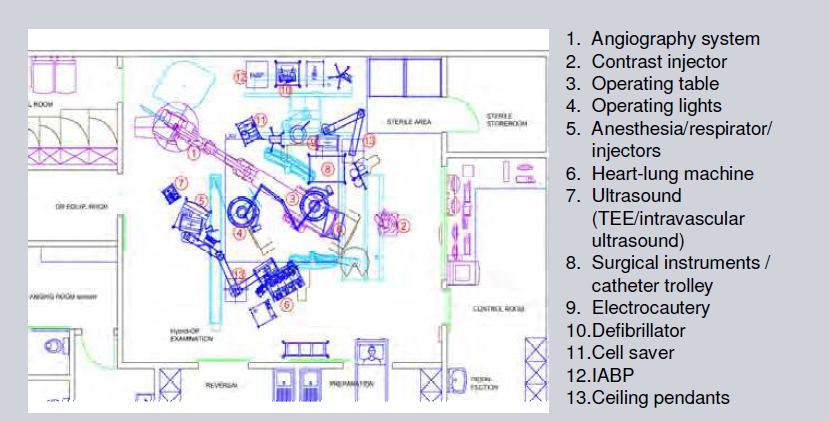
\includegraphics[scale = 0.7]{Content/Pictures/roomplanning.png}
	\caption{Beispielhaftes Layout für die Planung eines Hybriden OP-Saals \cite{HybridOR}}
	\label{fig:roomplanning}
\end{figure}

\subsection{Kosten- Nutzen Verhältnis}

Eine der Fragen die noch geklärt werden muss, ist ob ein Hybrider OP-Saal tatsächlich den Mehraufwand an Kosten und Umstrukturierung lohnt. Die benötigte Raumgröße und Ausrüstung führen dazu, dass ein Hybrider OP-Saal in der Anschaffung mehr als doppelt so teuer und in der Wartung fast doppelt so teuer wie ein Konventioneller OP-Saal ist \cite{HybridOR}. Gleichzeitig hat sich herausgestellt, dass neue medizinische Technologien bereits positiv aufgenommen werden, obwohl ein Mehrwert dieser noch gar nicht bewiesen wurde. Dies und die Digitalisierung des Operationssaals, hat in den letzten Jahren zu erheblichen Steigerung der Gesundheitskosten beigetragen \cite{DerDigitaleOperationssaal}. \\
Welchen Mehrwert ein Hybrider OP-Saal tatsächlich bringt wird in Bezug auf Kosten und Operationszeit überprüft.

Im Anwendungsfall des Bauchaortenaneurysma konnte eine Operationszeiteinsparung von 23,5 Minuten (von 120 auf 96,5 Minuten), mit einem Hybriden OP-Saal gegenüber einem Konventionellen mit C-Bogen, erreicht werden. Die Zeiteinsparung führt zusätzlich auch zu einer Einsparung der Prozesskosten und beträgt 276,17€ weniger pro durchgeführte Operation. Bei dieser Studie wurden jedoch Ergebnisse eines konventionellen OPs mit 97 Patienten von 2007 bis 2010 und beim Hybriden mit 50 Patienten von 2012 bis 2015 verglichen. Ein positiver Trend ist dennoch zu verzeichnen, da bei den Patienten und dem Operationsteam sehr auf  ähnliche Charakteristika geachtet wurde \cite{HybriderVsKonventioneller}.\\
Durch die Operationszeiteinsparung im Hybriden OP-Saal ist also tatsächlich eine Refinanzierung möglich \cite{HybriderVsKonventioneller}. Hinzu kommen positive Ergebnisse ohne einen direkten Vergleichswert, wie beispielsweise bei der Tumorentfernung. Bei 14 aus 16 Fällen konnten die Tumore komplett entfernt und mögliche auftretende Brain Shifts frühzeitig erkannt werden \cite{BrainShiftInTumorResection}.

Da Studien zum Vergleich zwischen einem Hybriden und Konventionellen Operationssaal zum einen kaum vorliegen und zum anderen schwierig durchzuführen und zu validieren sind, lässt sich die Frage des tatsächlichen Nutzens sehr schwer beantworten. Auch Todesraten sind kein Aussagekräftiges Ergebnis, da Überleben auch mit Lebensqualität zusammenhängt\cite{HybriderVsKonventioneller}. \\
Weitere wichtige Faktoren, die einen Einfluss auf den Nutzen haben, sind die gefühlte und tatsächliche Sicherheit von Patienten und Chirurgen. Die psychologische Seite ist jedoch noch schwieriger zu bewerten als das tatsächliche objektive Ergebnis \cite{DerDigitaleOperationssaal}.

Trotzdem lässt sich festhalten, dass der Hybride OP-Saal seine Vorteile mit sich bringt. Nicht in allen medizinischen Bereichen wird er einen gleichgroßen Nutzen zur Geltung bringen es eröffnen sich neue Möglichkeiten zur Operationsdurchführung. Somit stellt der Hybride OP-Saal die Grundlage für die Zukunft der Chirurgie \cite{ORofTheFuture}.





 





